\documentclass[12pt,oneside]{CUNY_PhD}

\pagestyle{headings}
\title{Finite Gaussian Neurons - A Defense Against Adversarial Attacks?
}
\author{Felix Grezes}

% \usepackage{fullpage}
\usepackage{graphicx}
\usepackage{amssymb}
\usepackage{url}
\usepackage{epstopdf}
\usepackage{enumitem}

%% ...
%% any 'preamble' stuff
%% ...


\begin{document}

\frontmatter

\maketitle % same name as the 'book' documentclass command, but gives a CUNY titlepage

%% optional:
\makecopyrightpage

\makeapprovalpage{1st Committee member}{2d Committee member}{3d Committee member}{4th Committee member}

%% optional:
\makeabstractpage{Pr. Michael I. Mandel}{Text of Abstract, up to 350 words}

%% (In addition to these last four custom CUNY commands, all LaTex
%% commands, including those from the LaTeX 'book' class, are available.
%% Footnotes and the bibliography will be single spaced, as
%% required by CUNY, while the main text will be double spaced.)

%% optional:
\chapter*{Acknowledgements}
%% Text of acknowledgements

\tableofcontents

\mainmatter

\chapter{Introduction}

\chapter{Background}
\section{Neural Networks}
\subsection{Particulars of Neural Networks for Vision}
\subsection{Particulars of Neural Networks for Audio}

\section{Adversarial Attacks on Neural Networks}
\subsection{Visual Adversarial Attacks}
\subsection{Audio Adversarial Attacks}

\section{Proposed Work}
\subsection{Main Idea: Finite Gaussian Neuron Activity}
%Intuition, Math, Advantages to other counter-measures
A typical artificial neuron's output $y$ is defined by its inputs $x_i$ and associated weights $w_i$ as: 
\[ y = \varphi(\sum_{i}w_i x_i) \]
with $\varphi$ being the non-linear activation function required by the universal approximator theorem \cite{cybenko1989approximation, hornik1989multilayer}. Usually a bias term is included, but it can be written as an extra input with value 1. 

\begin{figure}[!htbp]
\centering
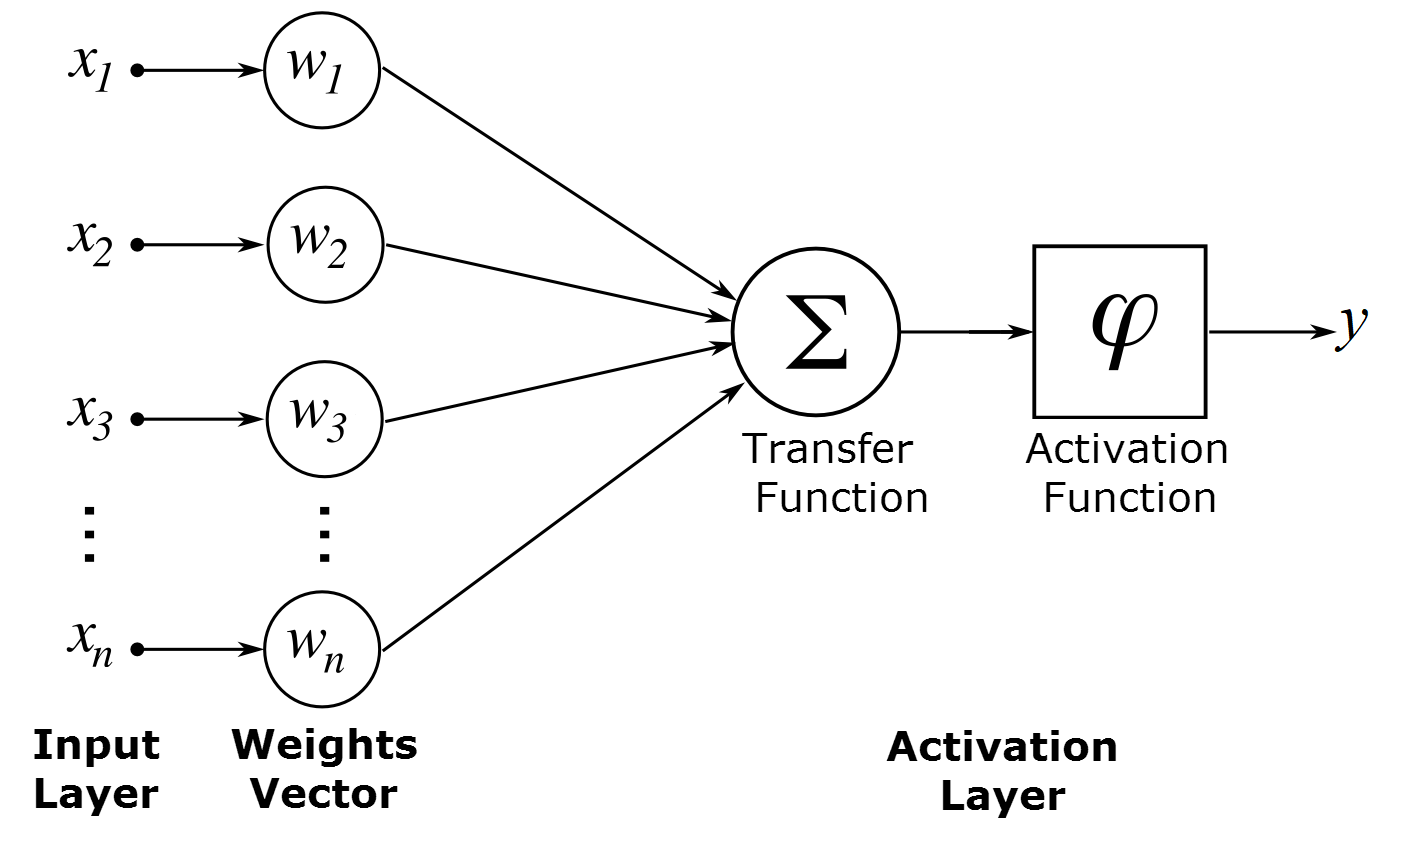
\includegraphics[width=0.9\textwidth]{images/artificial_neuron_model.png}
\caption{Model of an Artificial Neuron}
\label{fig:neuron}
\end{figure}

The $x_i$ inputs times $w_i$ weights product defines an underlying linear activity gradient over the input space, which is theorized to be a reason adversarial attacks on neural networks are effective \cite{46153}. An visual example of the linear activity over a 2D input space is given by \ref{fig:linmap}.

\begin{figure}[htb]
\centering
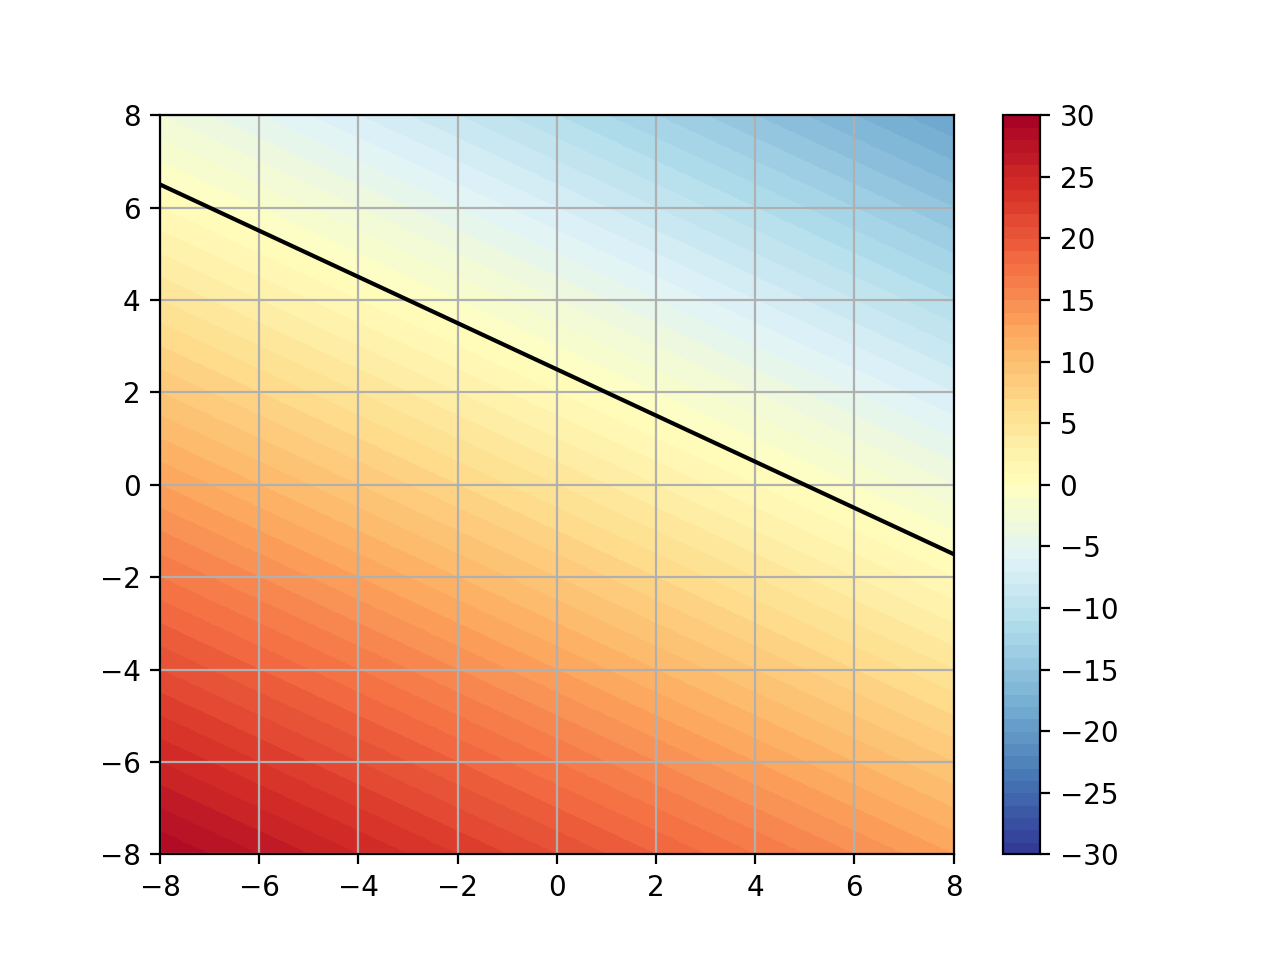
\includegraphics[width=0.9\textwidth]{images/2d_linear_map.png}
\caption{Underlying Linear Activity Map for a 2D Neuron}
\label{fig:linmap}
\end{figure}

To counter the locally linear decision boundaries of neural networks, I propose a modified neuron architecture, the Finite Gaussian Neuron (FGN). The output $y$ of a FGN is the $x_i$ inputs times $w_i$ weights product, multiplied by a circular Gaussian with learned mean and variance parameters:
\[ y = (\sum_{i}w_i x_i)*e^{(-1/\sigma^2)*(\sum_{i}(x_i-c_i)^2)} \]
% TODO draw fig:neuron but with gaussian side product
with $\sigma$ the learned mean and $c_i$ the learned center per input dimension. An visual example of the localized activity over a 2D input space is given by \ref{fig:locmap}. \\
Note that the circular Gaussian provides both the non-linearity and the bias term of classical artificial neurons. Both of which are needed for the universal approximator theorem for neural networks \cite{}.

% Proof of above statement
$\varphi (\cdot )$ needs to be a nonconstant, bounded, and continuous function.\\
We can write the activity of a LGN as:
\[ y = (\sum_{i}w_i x_i)*e^{(-1/\sigma^2)*(\sum_{i}(x_i-c_i)^2)}\]
\[y = w_Tx * \]

\begin{figure}[!htb]
\centering
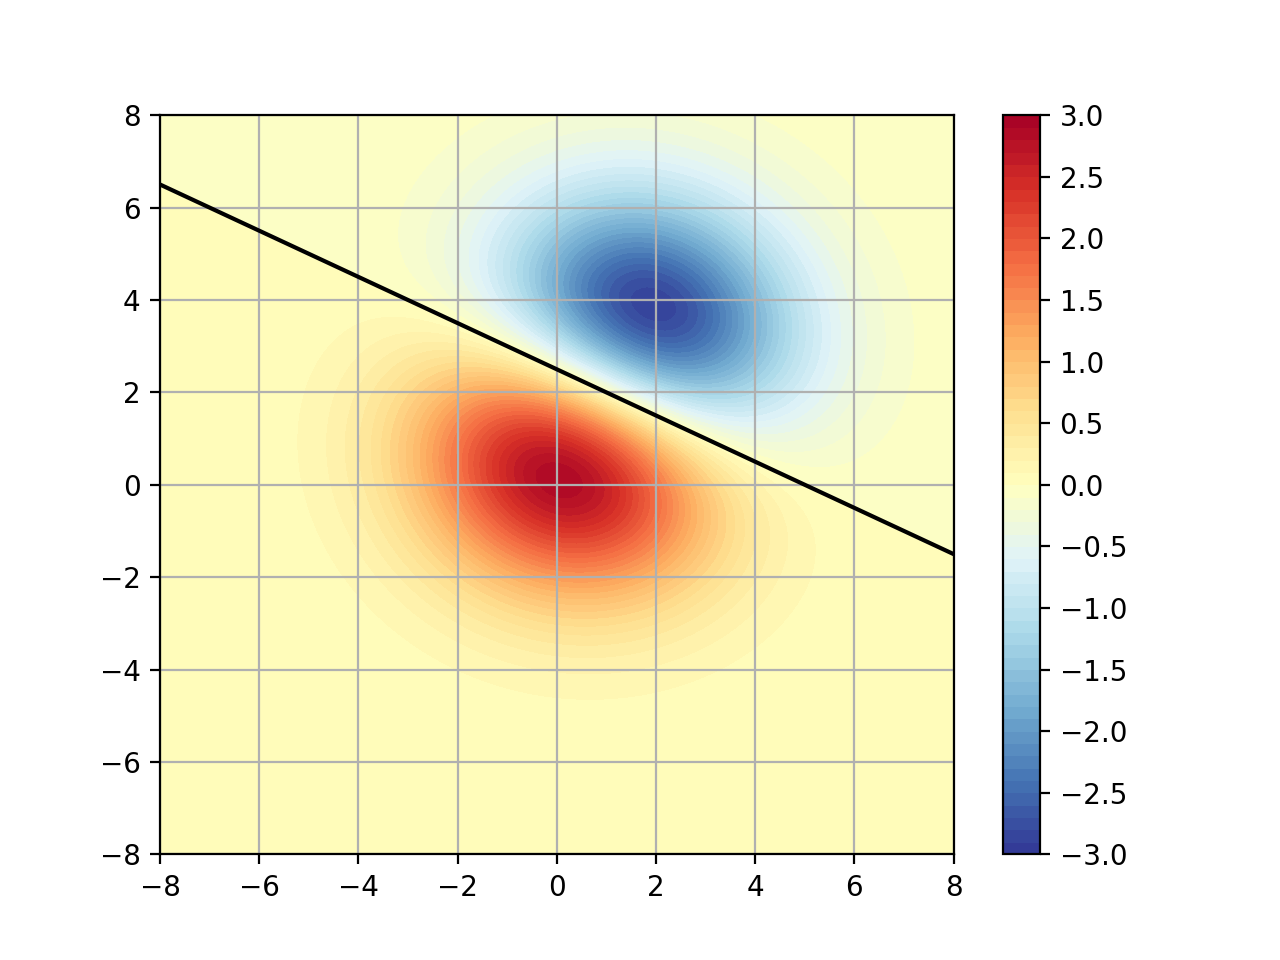
\includegraphics[width=0.9\textwidth]{images/2d_localized_activity_map.png}
\caption{Localized Activity Map for a Proposed 2D Neuron}
\label{fig:locmap}
\end{figure}

\subsection{Task 1: Visual}
% data, experiments, results
\subsection{Task 2: Audio}


%% If you want an introduction in the table of contents, but
%% without its own chapter number, do this:
%% \chapter*{Introduction}
%% \addcontentsline{toc}{chapter}{\numberline{}Introduction}
%% \markboth{Introduction}{INTRODUCTION}

%% Also, to ensure that the bibliography is in the table of
%% contents, do this when you reach the end of the main text:

\backmatter
%% \begin{thebibliography}{n} %(where n is the longest item)
%% \addcontentsline{toc}{chapter}{\numberline{}Bibliography }

\bibliographystyle{IEEEtran}
\bibliography{bibl.bib}


\end{document}